% You must put english here to handle hyphenation correctly
% Please keep this line to avoid using the parameter from the previous article in the proceedings
\selectlanguage{english} % possible values : french, english

\settitle[Runtime Security Monitoring with eBPF]{Runtime Security Monitoring with eBPF}

\setauthor[G.~Fournier, S.~Afchain, S.~Baubeau]{Guillaume Fournier, Sylvain Afchain \and Sylvain Baubeau\\
  \email{gui774ume.fournier@gmail.com\\sylvain.afchain@datadoghq.com\\sylvain.baubeau@datadoghq.com}}

\institute{Datadog}

% To handle authors with multiple institutions, you can use the following code:
%
%   \setauthor[M.~MonNom, A.~MonAutreNom]{MonPrenom MonNom\inst{1} \and AutrePrenom AutreNom\inst{2}\\
%     \email{monprenom.monnom@mycorp.com\\autreprenom.autrenom@mycorp.com}}
%
%   \institute{OrganismePourMonNom \and OrganismePourAutreNom}
%
% For \institute, the numbering is automatic (and starts at 1)


\maketitle
\index{Fournier, G.}
\index{Afchain, S.}
\index{Baubeau, S.}

\begin{abstract}
  From containerized workloads to microservices architecture, developers are rapidly adopting new technologies that allow organizations to scale at unprecedented rates.
  Unfortunately, fast mutating architectures are hard to keep track of, and runtime security monitoring tools are now required to collect application level and container level context in order to provide actionable alerts.
  This paper intends to explain how eBPF\footnote{The Extended Berkeley Packet Filter is a tracing technology in the Linux kernel. See section~\ref{section:RuntimeSecurityMonitoringWithEBPF:EBPF} for an in-depth presentation.} has made it possible to create a new generation of runtime security tools with significantly better performance, context and overall signal to noise ratio compared to legacy tools like AuditD\@.
\end{abstract}


\section{Introduction}

According to the Cloud Native Computing Foundation, container usage in production has increased by 300\% between 2016 and 2020~\cite{RuntimeSecurityMonitoringWithEBPF:CNCF}.
In other words, organizations are progressively moving away from static and dedicated infrastructures, and shifting towards micro-services and containerized workloads.
Container orchestration tools like Kubernetes are playing a key role in this trend, and security teams need to adapt their threat models and runtime detection capabilities to account for an infrastructure that is constantly changing.

One of the goals of a container orchestration tool like Kubernetes is to improve the usage of the resources available to a cluster.
More specifically, this means making sure that CPUs, memory and network bandwidth are better utilized and distributed among the services running on a cluster~\cite{RuntimeSecurityMonitoringWithEBPF:DevopsWithK8s}.
In order to achieve this goal, Kubernetes is able to mutate the infrastructure continuously so that workloads are better distributed among the hosts of the cluster, thus making sure that one machine is not saturated when another one can help share the load.
From a security standpoint, this means that multiple services can now run side by side at any point in time\footnote{Kubernetes can be configured to dedicate some hosts to specific workloads, but this requires a custom setup that often voids the entire point of a Kubernetes environment.
In this document, we expect Kubernetes to follow its default configuration, which is to allow any workload to be scheduled on any host of a cluster.}, sharing the same kernel, and increasing the blast radius in case of a compromise.
Not only does it blow up the impact of an intrusion, this also makes the life of the incident response team much harder, especially if the runtime monitoring tool that detected the attack did not provide accurate and real time information about the containers and the applications that were breached.

This paper proposes to explore eBPF to implement a new generation of runtime security tools, showing how this new technology can be used to retrieve complex container and application level context.
Although containers are a particularly interesting use case for the solution we implemented, we will also demonstrate how eBPF drastically improves the legacy runtime security tools that are used in production environments today, by reducing the performance impact on the host, improving the signal to noise ratio, and helping incident response team focus on what matters.

\section{Runtime security: state of the art}

Before we get into the details of the solution we came up with, we are going to better explain what we are trying to achieve and the limitations of the existing runtime security tools that we are trying to address.

\subsection{What is runtime security and why is it so important ?}

Runtime security is the ability to detect Indicators of Compromise (IOC) at runtime, in an attempt to alert your incident response team as soon as possible, and deploy countermeasures.
In more concrete terms, this vague statement translates into multiple layers of security that can be combined to reduce the probability of an attack slipping through your fingers, regardless of all the security measures taken during the development phase of your application, or the configuration of your infrastructure.
For example, at the infrastructure layer, Network Intrusion Detection Systems (NIDS) are often positioned at critical places in an infrastructure, to detect abnormal network activity, or known malicious network signatures.
At the host level, Host Intrusion Detection Systems (HIDS) are usually deployed to detect abnormal process behaviors, or suspicious resource usage.
An HIDS with prevention capabilities would be classified as an Host Intrusion Prevention System (HIPS).
Add a backend to gather alerts and match the collected events against a threat intelligence database, and the HIDS is now part of an Endpoint Detection and Response (EDR) platform.
Then if you go one layer deeper, at the application level, Web Application Firewalls (WAF) are often deployed as a middleware before your web applications, in an attempt to detect and block abnormal requests before they reach a service.
And if you finally reach the code level instrumentation, you’ll find Runtime Application Self-Protection (RASP) tools.
The main difference between a WAF and a RASP is the ability of the instrumentation to understand how the application will react to a specific attack signature.
For example, while a WAF would block an SQL injection attempt unconditionally, a RASP would be able to detect if the injected query will be properly escaped or executed.
Our approach sits right in the middle of an HIPS and an EDR.
Our hypothesis is that analyzing system level events has the best chance of catching malicious behaviors without requiring special application level instrumentation (and therefore becoming a burden to developers), or conceding coverage and detection capabilities to performance concerns and mutating infrastructures.

IOCs come in multiple shapes and sizes.
Since this paper is about Host Intrusion Detection Systems, we are going to give examples of host based indicators only.
For example, a host based IOC can be as simple as: "a process, that is not your web server, read a sensitive file that contains credentials to your SQL database", or "an interactive shell was spawned by a web server".
A more complex example could include containers: "a docker client was started from within a container".
IOCs can also be dedicated to specific vulnerabilities, thus helping to detect the exploitation of known vulnerabilities in an infrastructure.
When it comes to runtime security, the limitations with IOCs usually come from the HIDS: is it versatile enough to collect the right data for the IOC to be detected ?
Most importantly, IOCs, by themselves, will tell you that a vulnerability might have been exploited, but what really matters to an incident response team, is the context provided by the HIDS to understand what happened, how critical the situation is and what needs to be patched.
In other words, you may have the best IOCs, and the best incident response team, if your HIDS does not follow suit and is limited in either the context it provides or its detection capabilities, the impact of the runtime security team will be severely limited.

Apart from the application of good security practices like defense in depth, runtime security is also made necessary by the increasingly problematic struggles of application security.
In a few words, application security includes all the steps taken by a security team to ensure that the services developed by an engineering team are not inherently flawed.
From code security reviews and developers security training, to third party dependency scanning, many layers can be introduced and automated to catch vulnerabilities before they make their way into production.
Although application security is an absolutely crucial part of the security of an organization, it is, more realistically speaking, an attempt at reducing the frequency and the blast radius of security incidents, rather than a bullet proof strategy.
The truth is, application security is an almost impossible task:

\begin{itemize}
  \item Security teams will never have enough context and visibility into the pieces of software under active development to properly review and validate all implementation designs.
  \item Third party dependency scanners are by definition telling you about vulnerabilities that are already publicly known and potentially under active exploitation.
  \item Zero days are a thing.
  \item Vulnerability management is complicated, and medium vulnerabilities can pile up more quickly than you think.
\end{itemize}

From an application security analyst perspective, another very frustrating fact is to discover a vulnerability in production and painfully realize that it will take weeks if not months to patch it.
Many things can get in the way.
Taking an entire product offline to patch a vulnerability isn’t always an option.
Developers are under constant pressure to produce new features.
All hands on deck situations need to be carefully weighed.
And even when developers are actively working on a solution, there is a coverage gap between the moment when a vulnerability is discovered in an application and when the security patch is actually deployed.
During this coverage gap, the application security team is effectively powerless.
The rise of containers have even accentuated the problem.
Indeed, most organizations that use containers at scale will set up container build pipelines to control their base image instrumentations, and unify their ecosystem.
Should a vulnerability be discovered in a key component of the base image, this is suddenly the entire infrastructure that is at risk.
One could think that such pipelines would actually be beneficial and ensure that a patch is deployed in a timely manner, and more importantly, deployed everywhere.
Unfortunately, experience has shown that the maintainers of those base images are comprehensively reluctant to update them, in fear of suddenly breaking builds for the entire company.
In short, application security analysts are playing catch up at a game that is becoming increasingly hard to win in a containerized world.

This is where runtime security comes in.
The ability to understand how your workloads behave, and to detect exploitations at runtime is the natural continuation of application security.
The tool we are presenting here has a customizable rule engine that can, among other use cases, be used to deploy dedicated IOC detectors, so that security teams can be made aware of the active exploitation of a known vulnerability.
More on that in the following sections of this paper.

Another strong incentive to runtime security is compliance.
Many compliance standards like the Payment Card Industry (PCI) standard have File Integrity Monitoring requirements (see requirement 11.5~\cite{RuntimeSecurityMonitoringWithEBPF:PCI}).
In a nutshell, those requirements demand that sensitive system files and files containing credentials or any other sensitive information be actively monitored for modification and access.
These use cases are included in runtime security and behavioral analysis.


\subsection{Existing runtime security tools have problematic limitations}

Unfortunately, runtime security is far from being a solved issue.
During our research, we’ve identified a few major limitations with which most existing solutions struggle.
It is also important to note that those limitations are usually inherited from the runtime monitoring technology that powers the tool.
What we call runtime monitoring technology is simply the data source used by the HIDS.
For example, go-audit~\cite{RuntimeSecurityMonitoringWithEBPF:GOAudit} is powered by the Audit Framework~\cite{RuntimeSecurityMonitoringWithEBPF:LinuxAudit} of the Linux kernel. Similarly, the File Integrity Monitoring feature of Wazuh~\cite{RuntimeSecurityMonitoringWithEBPF:Wazuh} or Auditbeat~\cite{RuntimeSecurityMonitoringWithEBPF:AuditBeat} are powered by Inotify~\cite{RuntimeSecurityMonitoringWithEBPF:FilesystemNotification}.
Go-audit will therefore inherit the limitations of the Audit Framework, and similarly Wazuh or Auditbeat will necessarily be limited by the capabilities of Inotify.
This is why we focused our research on the most used runtime security monitoring technologies, instead of trying to assess all the existing HIDS on Linux.

Out of all the runtime security technologies we’ve looked at, the most represented ones are (not in any particular order):

\begin{itemize}
  \item The Linux Audit Framework
  \item Inotify and fanotify~\cite{RuntimeSecurityMonitoringWithEBPF:Fanotify}
  \item Netlink based process events, coupled with the proc filesystem for context
  \item Periodical checks with file hashes or known signatures
  \item A custom kernel module
  \item Perf events coupled with kprobes~\cite{RuntimeSecurityMonitoringWithEBPF:KprobeDocumentation} or other kernel hook points technology
  \item Ptrace (sometimes coupled with seccomp-bpf filters), we won’t talk much about this one because of the obvious performance drawback of a solution that interrupts the execution of a program at each syscall and duplicates the amount of context switches.
  That said, a few projects did try to use it.
\end{itemize}

Instead of going through them one by one, we believe that it is a lot more valuable to discuss how their limitations affect the runtime detection capabilities.
More importantly, we want to understand the compromises a security team would have to make in order to use an HIDS based on each one of them.

\subsubsection{Context}

The first and most important challenge is the context provided by the runtime technology.
Without context, incident response teams will struggle to triage and take action on the alerts.
The most relevant example of this limitation is File Integrity Monitoring use cases.
Runtime security teams are very likely to want to collect accesses to sensitive credential files like "/etc/shadow" or "/etc/passwd".
The problem is that those files can be accessed legitimately by processes like "docker", "systemd" or even "passwd" when a new user is added to a host.
If your HIDS is based on Inotify or periodical checks, you won’t get any context on the process that touched the file.
In other words, your runtime security team will constantly get paged, without really understanding what happened.
Eventually, the alerts will be considered as noise, and the team will have to stop looking at them.
Similarly, the detection capabilities of such an HIDS are limited: the only IOCs that a runtime security team will be able to detect will have to be file system related.

Process context is not the only context that runtime security monitoring technologies struggle with.
Container context is also a pretty widespread issue.
The main reason that explains this struggle is that containers are a user space concept, which translates in kernel space into namespaces and cgroups.
Matching namespaces and cgroups to container metadata needs to be at the core of the runtime security monitoring technology for the detection to be efficient and contextualized.
Simply put, out of the entire list of runtime technologies, only 2 have the ability to reliably support containers for both context and detection use cases: a custom kernel module and eBPF.
It is also important to note that many workarounds have been attempted to support containers.
The most represented attempt is a fall back to the proc filesystem to retrieve the container ID of a process by looking at its cgroup path.
This solution has been attempted by solutions based on the Audit Framework~\cite{RuntimeSecurityMonitoringWithEBPF:GOAuditContainerID} or \emph{perf} (Capsule8’s sensor used to do it, but their project is no longer publicly available).
Unfortunately, this solution is a best effort workaround that introduces many security concerns, especially reliability problems for short lived processes.
Indeed, by the time an alert is handled by the user space part of the HIDS, the malicious process may no longer be available through the proc filesystem.

Container context is crucial to runtime security teams for 2 main reasons:

\begin{itemize}
  \item In a containerized infrastructure, workloads can come and go at any moment on a host, following the orders from the scheduler of the containers orchestrator.
  This means that, although knowing the process that triggered an alert is crucial, knowing from which container (if any) the alert was triggered will help the security team narrow down their research to the service(s) running in that container.
  Without this knowledge, a wild witch hunt would have to be undertaken, and precious time would be wasted.
  \item Container level detection capabilities.
  Without the ability to reliably collect container metadata at runtime, an HIDS cannot detect IOCs based on them.
  A commonly used example is the detection of the Graboid~\cite{RuntimeSecurityMonitoringWithEBPF:Graboid} crypto jacking worm.
  One of its most important IOC is the execution of the docker client within a container.
  \item Similarly, container escape IOCs necessarily require the knowledge that a process was initially inside a container.
\end{itemize}

\subsubsection{Signal to noise ratio and coverage loss}

Part of this point is a direct consequence of the previous one.
The less context an HIDS has access to, the less accurate it will be.
For a runtime security team, this means having to deal with a growing number of alerts, and ultimately having to tune down an IOC or even turning it off entirely.
To go back to the "/etc/passwd" example, you may be tempted to filter out the processes that accessed the file without a TTY.
This way, you would be notified only when an actual person tried to access the file instead of a service in production.
Unfortunately, this introduces a dangerous blind spot that can be easily exploited to bypass detection.
In short, a solution with limited context will produce noisy alerts and force the security team to either ignore them or turn them off.
In both cases, coverage loss is inevitable.

Apart from context, some runtime security monitoring technologies struggle with technical limitations which ultimately lead to coverage loss.
An obvious example is the use of the proc filesystem for process context.
We’ve already talked about it: short lived processes might already have died by the time the user space part of the HIDS queries the proc file system for context.
Another less obvious example is related to \emph{perf} events~\cite{RuntimeSecurityMonitoringWithEBPF:Perf}.
Configured with a kprobe, the \emph{perf\_event\_open} syscall can be used to ask the kernel to dereference a kernel structure and collect data at precalculated offsets.
For example, this can be used to collect the path provided to the \emph{open} syscall and therefore to implement a basic File Integrity Monitoring tool.
Unfortunately, this method has hidden limitations which may lead to coverage loss.
Indeed, \emph{open} syscalls can be given relative and unresolved paths.
In other words, the input cannot be reliably used as a trusted source for your detection.
If you wanted to collect the resolved path with \emph{perf}, you would have to hook much deeper in the kernel, and dereference the file system \emph{dentry}~\cite{RuntimeSecurityMonitoringWithEBPF:Dentry} tree to retrieve the resolved path one parent at a time (this method is described in more details in the last part of the document).
The bad news is that the kprobe interface is limited in the amount of times it can dereference a structure, which ultimately leads to a maximum resolved path depth of 9 (the limitation is ultimately due to the fact that the kprobe interface requires that arguments be below MAX\_ARGSTR\_LEN~\cite{RuntimeSecurityMonitoringWithEBPF:KprobeInterface} in length).
In other words, there are hard limitations to some runtime security monitoring technologies that may have severe consequences on the capacity of said technology to be used in a security tool.

Note that eBPF has hard limitations as well.
For example, the most constraining one is that the total count of instructions of an eBPF program must be below 4096.
This limit was raised in newer kernel versions to 1 million (kernels 5.1+~\cite{RuntimeSecurityMonitoringWithEBPF:VerifierScalability}).
Fortunately, so far we’ve been successful in working around those limitations in a way that does not impact our coverage capabilities or performance footprint.
More on that in the following sections.

\subsubsection{System overhead and resources usage}

Another reason that may compel a security team to tune down its detection rules is the performance of the HIDS and its overall footprint on a host.
When evaluating the performance impact of an HIDS, there are always 2 types of overheads to take into account.
The first one is the latency introduced in the kernel because of the runtime security monitoring technology in use.
For example, we could argue that activating AuditD has a bigger impact on the kernel than activating inotify watches on a few well defined files, because of the limited granularity of the AuditD rule engine.
The second one is the resources required by the user space application to handle the events retrieved from the runtime security monitoring technology.
From our experience, the most noticeable impact on a host comes from the number of times an event has to be sent to user space, and the amount of work that needs to be done in user space to handle this event.
In other words, the earlier an event can be confidently dropped and ignored, the better.
This is why programmable solutions like eBPF or kernel modules are particularly interesting.
Having the ability to develop fine grained in-kernel filter to control the amount of data sent from kernel space to user space is a game changer.

\subsubsection{System safety}

It was probably obvious from the beginning that kernel modules would be one of the top contestants in the search for the most powerful way to instrument the Linux kernel.
However, from a runtime security team perspective, kernel modules have one major problem: they require a very high level of trust in their stability.
Indeed, a crash of a kernel module would immediately crash the host, thus threatens the availability of the service that the security team is trying to protect.
Not only can this have security and compliance consequences, it will also make it really hard for a security team to get an infrastructure team onboard with the deployment of a solution that might crash an entire system.
In comparison, eBPF has a key feature which ensures that the program pushed in kernel space cannot cause a kernel panic: the eBPF verifier.
We'll get into more details about it in the next section.

\section{What is eBPF and what can you do with it ?}
\label{section:RuntimeSecurityMonitoringWithEBPF:EBPF}

Since its first appearance in 2014 (Kernel 3.15)~\cite{RuntimeSecurityMonitoringWithEBPF:VirtualMachine}, BPF has progressively become a key technology for observability in the Linux kernel~\cite{RuntimeSecurityMonitoringWithEBPF:BrendanGregg}.
Initially dedicated to network monitoring, eBPF can now be used to monitor and trace any kind of kernel space activity.
eBPF is still under active development and new features are regularly announced.
One particularly interesting and recent addition to the kernel is the Kernel Runtime Security Instrumentation (KRSI)~\cite{RuntimeSecurityMonitoringWithEBPF:KRSI} which introduces the ability to implement a Linux Security Module (LSM)~\cite{RuntimeSecurityMonitoringWithEBPF:SecurityModule} with eBPF.

\subsection{Overview of eBPF}

This section is an overview of the Extended Berkeley Packet Filter (eBPF) subsystem within the kernel.
Its architecture is so complex that we are not going to deep dive into all its inner workings.
Instead, we are going to provide the key principles on which eBPF is built, so that the reader understands how this technology works and how it can be used to instrument the kernel with a security use case in mind.

The first thing you need to know is that eBPF programs run in a virtual machine within the Linux kernel.
Compilers like LLVM and GCC provide support for BPF, allowing a C program to be compiled into BPF instructions.
Once compiled, an eBPF program is loaded in the kernel using the \emph{bpf} syscall.
As mentioned in the previous section, multiple steps were taken to ensure that eBPF programs cannot cause a kernel panic.
One of these steps is called the eBPF verifier.
When the program is loaded in the kernel, the eBPF verifier checks that the program complies with multiple limitations imposed to eBPF.
For example, the stack of each eBPF program cannot exceed 512 kilobytes, loops are forbidden (although they were recently added for kernels 5.4+~\cite{RuntimeSecurityMonitoringWithEBPF:Loops}), more precisely, the verifier checks that your program is a Directed Acyclic Graph (DAG), the maximum number of instructions per program is limited (4096 instructions for kernels up to 5.4 and then 1 million instructions~\cite{RuntimeSecurityMonitoringWithEBPF:VerifierScalability}), many other restrictions apply to memory accesses.
Although those limitations might seem extremely restrictive, they are the reason why eBPF is so popular in tracing and monitoring tools.
Indeed they ensure the safety of a program and that its overhead on the system will remain low.
Once a program is verified, the kernel uses a just-in-time (JIT) compiler for BPF instructions to transform the BPF bytecode into machine code.

Once you’ve loaded an eBPF program, you need to tell the kernel how and when the program should be triggered.
Multiple eBPF program types were introduced over time and each has its own use case~\cite{RuntimeSecurityMonitoringWithEBPF:LorenzoDavid}.
Some are dedicated to network use cases while others can be used to hook onto any exported symbol of the Linux Kernel.
With a security use case in mind, it is interesting to know that some program types have enforcement capabilities (like the ability to drop a network packet) while others are only dedicated to tracing use cases.
To give a concrete example, the kernel Kprobe interface can be used to attach an eBPF program to specific symbols in the kernel.
This ensures that the eBPF program will be called anytime this symbol is called (on entry or exit of the function).
In more technical terms, when an eBPF program is attached to a kernel symbol, the kernel inserts at runtime a trampoline at the beginning or end of the function, so that the execution jumps into the eBPF program, thus letting it access the input parameters of the function, or its return value.
Apart from the arguments of the function call, many BPF helper functions can be used to gather additional runtime context.
This context can be as simple as the process and thread ID that is currently executing the function.
More complex eBPF helpers can be used to retrieve the user space stack trace of the program that triggered the execution of the kernel function.

eBPF is also armed with multiple storage mechanisms that can be used to communicate with a user space program.
Just like eBPF programs, eBPF maps come in many different shapes and sizes.
The good news is that the verifier does not count the memory allocated by an eBPF map as part of the stack of an eBPF program.
eBPF maps are usually used for two things:

\begin{itemize}
  \item Collecting kernel space data and exposing it to a user space.
  With the right access, a user space program may query a map and dump its content.
  \emph{Perf} ring buffers can also be used to send a stream of events to user space in a particularly efficient way.
  \item Pushing data from user space to kernel space.
  From an HIDS use case perspective, this is how in-kernel filters can be pushed to configure your eBPF programs and let them know what kind of events you are interested in.
\end{itemize}

Other more complex eBPF maps have dedicated use cases.
For example, LPM\_TRIE can be used to figure out the subnet mask of an IP address.
PROG\_ARRAY maps can be used to tail call your eBPF programs.
In a nutshell, this features makes it possible for an eBPF program to programmatically decide to call another eBPF program.
This helps workaround the instructions count limitation because tail calling can be done up to 32 times.

Another interesting upcoming addition to the kernel is the ability to sign eBPF programs~\cite{RuntimeSecurityMonitoringWithEBPF:SignedBPF}.
This will help make sure that only verified eBPF programs can be loaded at runtime.

Many other rules apply to eBPF, but the few principles exposed above should be more than enough to grasp how powerful eBPF is, and how we used it to implement our HIDS.

\subsection{eBPF and security use cases}

The most natural security use case of eBPF is network security monitoring and enforcement.
This is simply because network packet filtering was the reason why the BPF virtual machine was initially added to the kernel.
Many popular packet filtering tools are based on eBPF.
For example, bpfilter should eventually replace iptables in the linux kernel~\cite{RuntimeSecurityMonitoringWithEBPF:Firewall}.
Complex network security monitoring and enforcement tools were also built on eBPF.
Cilium and Cloudflare are only two of the biggest examples out there.
Last year, we presented at SSTIC 2020 a much deeper analysis of what eBPF can do for network security monitoring and enforcement~\cite{RuntimeSecurityMonitoringWithEBPF:NSP}.

In a recent addition to the kernel (kernel 5.8+), Google contributed the Kernel Runtime Security Instrumentation (KRSI)~\cite{RuntimeSecurityMonitoringWithEBPF:KRSI}.
This is the first major push towards a runtime security use case (other than network) implemented for the eBPF subsystem.
In a nutshell, the patchset submitted by Google introduces a new program type that leverages Linux Security Module (LSM)~\cite{RuntimeSecurityMonitoringWithEBPF:SecurityModule} hook points to implement a dynamic Mandatory Access Control with eBPF programs.
This technology will essentially bring enforcement capabilities to any HIDS based on eBPF, thus turning them into HIPS.
Furthermore, hooking at the LSM level has many benefits such as hook point stability insurances or the guarantee that your programs will always be called on certain types of resource access requests.
We’ll see in the next section why an HIDS based on eBPF without KRSI is particularly susceptible to those two kinds of bypasses.
Unfortunately, KRSI is a recent addition to the Linux kernel, which means that for now, HIDS solutions based on eBPF will have to work without it.

\subsection{What's the catch ?}

So far we’ve presented eBPF as being the safest, fastest and overall most flexible tracing and monitoring technology.
The truth is, eBPF has its fair share of limitations which can have dangerous consequences for an HIDS.

The first issue isn't exactly introduced by eBPF, but rather by the Kprobe interface of the linux kernel.
This interface gives the possibility to attach eBPF programs on arbitrary hook points in the kernel.
The choice of those hook points would be at the core of an HIDS.
For example, in order to detect file accesses or process executions, you would have to hook on the functions that the kernel calls to either access a file system or execute a binary file.
Unfortunately, the kernel is always changing and from one kernel version to another, those hook points may change as well.
In other words, there is no guarantee that the hook points on which you based your detection will be available in a production environment that runs a different kernel version or Linux distribution.
Similarly, the kernel structures of the arguments of the hooked functions passed to your eBPF programs may change.
Depending on kernel build configuration parameters and on the kernel version, the offset of an attribute from the base address of a structure may change.
Ultimately, this means that the kernel headers you used in your CI to build your program might be drastically different from the kernel headers of your hosts in production.
Your eBPF programs would then retrieve invalid data, and your detection would essentially not work.
Compiling your eBPF programs at runtime with the headers of the host might fix the issue but it may not always be an option.
A recent initiative called Compile Once - Run Everywhere (CO-RE)~\cite{RuntimeSecurityMonitoringWithEBPF:CORE} should solve this problem by introducing a new metadata format~\cite{RuntimeSecurityMonitoringWithEBPF:BTF} that can be used at load time to override the kernel offsets of an eBPF program with the correct values.
Unfortunately, this feature is quite hard to backport to kernel versions below 5.4.
In other words, hooking right in the middle of the kernel without any symbol stability guarantees is hard and can ultimately lead to detection bypasses if not handled carefully.

Therefore, the usual approach taken by eBPF based HIDS, such as Falco~\cite{RuntimeSecurityMonitoringWithEBPF:Falco}, is to hook at the syscall level.
Syscalls are more stable than deeper kernel hook points since changing them would immediately introduce breaking changes in user space programs, and it hasn’t happened so far.
However there are four dangerous problems with this approach:

\begin{itemize}
  \item The first one is that you need to be on the constant look out for new and rarely used syscalls.
  Indeed, forgetting to hook on a specific syscall may lead to entire bypasses of your HIDS.
  For example, in the context of a File Integrity Monitoring use case, you would need to hook on all the syscalls that can be used to open a file.
  You will obviously include the \emph{open} and \emph{openat} syscalls, but those 2 syscalls are not the only way to open a file on Linux.
  Two other less popular syscalls exist: \emph{open\_by\_handle\_at}~\cite{RuntimeSecurityMonitoringWithEBPF:OpenByHandleAt} and \emph{io\_uring\_enter}~\cite{RuntimeSecurityMonitoringWithEBPF:IOUring}.
  Those syscalls are much harder to support mainly because the file context is decoupled from the file access operation.
  This shows how dangerous it is to hook at the syscall level and explains why the Linux Security Module (LSM) interface exists: regardless of the call path, each resource handled by the kernel has its own LSM function to implement access control.
  In other words, hooking at the LSM level prevents call path bypasses.
  \item Another issue with working at the syscall level is that syscall calling conventions may change.
  This usually translates into having to insert multiple kprobes to hook on a single syscall.
  From one kernel to the next, those calling conventions might not always be there, so you’ll need to adapt your probes accordingly and be very careful to avoid bypasses.
  This issue is also why some eBPF powered tools usually move to tracepoints~\cite{RuntimeSecurityMonitoringWithEBPF:Tracepoints} instead of kprobes.
  Tracepoints are another interface that can be used to hook into the kernel, with the difference that they are maintained by the kernel developers manually.
  Tracepoints are therefore a stable hook point ABI, but consequently they are a lot less versatile and flexible than kprobes.
  \item The third issue with syscalls is that they might provide incomplete context.
  For example, an unresolved relative path like "./../../shadow" may be provided to an open syscall, and your eBPF program will have a really hard time understanding if you are actually opening "/etc/shadow" or not.
  Long story short, because of various eBPF limitations, it is actually impossible to resolve such a path to the real file, if you stay at the syscall level.
  This is a huge problem because this means that you’ll have to resolve the paths in user space, while also having to track the current working directory of all the processes on a host, as well as soft links, hard links and mount points.
  Except if you don’t care about in-kernel filtering and overall performances, this is not the way to do it.
  Another good example of the limited context that syscalls provide is the execve syscall.
  Apart from the path problem that also applies to this syscall, you might want to collect process credentials such as its user and group.
  However, when the syscall is called, the eBPF program will be triggered from the context of the parent process (since the execve syscall has not been executed yet), and therefore, the various eBPF helper functions will all yield context from the parent process.
  Should the executable be a setuid or setgid binary, the process context you’ll have to work with, will essentially be incorrect.
  For this specific example, moving to a probe on the return of the \emph{execve} syscall, would resolve the issue.
  \item The fourth and probably most problematic issue is that memory pointers provided to a syscall are vulnerable to Time-Of-Check Time-Of-Use attacks.
  If you read a user space memory buffer on entry of a syscall, there is no guarantee that the kernel will read the same data later in the call path.
  Indeed, a user space thread in the same process could swap the data in the buffer (right after the eBPF program is executed) with the real file path that the compromised process wants to open.
  The same limitation applies to syscall exit probes but in the reversed order.
  In other words: don't trust user space memory buffers, and do not collect sensitive data from user space pointers at the syscall level.
  \item If the previous point wasn't a strong enough incentive to avoid working with user space memory buffers, this final one might be: it isn't always possible to read user space memory buffers from eBPF.
  When a memory page isn't in RAM, the kernel would usually trigger a major page fault so that the data is loaded from the disk.
  Although eBPF programs are executed in kernel space, they are not authorized to trigger major page faults, thus to read user space memory pages that are not directly accessible from the RAM.
  In other words, an attacker could use this knowledge to hide malicious parameters from your eBPF programs.
\end{itemize}

So it seems that eBPF isn’t the easiest choice for a security use case: first, it is really hard to hook deep inside the kernel because of stability issues, second, hooking at a higher level and stable interface like syscalls might yield incorrect data.
The following section explains how we’ve solved both problems, and more importantly, how we’ve exposed a customizable rule engine that can be leveraged to write detection rules for complex IOCs.

\section{The Datadog Runtime Security Agent}

The Datadog runtime security agent~\cite{RuntimeSecurityMonitoringWithEBPF:DatadogAgent} is an open source HIDS powered by eBPF, that aims at detecting host level attacks in real time such as Remote Code Execution (RCE) attacks or credentials theft attempts.
Our goal was to provide an answer to the coverage gaps that we identified in the first section, while working around the limitations of eBPF listed in the second section.
We built this HIDS while keeping in mind the real world struggles that runtime security teams have to deal with on a daily basis.
In short, we believe that runtime security teams shouldn’t have to compromise with any aspect of runtime security: actionable alerts with container aware metadata, low performance impact and system stability, powerful and customizable detection capabilities with a high signal to noise ratio, etc.
Everything matters to prevent intentional or unintentional coverage loss.
These are engaging promises, and there is much to cover, so let’s get into it !

\subsection{High level overview}

At a high level, the runtime security agent is made of 3 different components:

\begin{itemize}
  \item Our eBPF programs, which we carefully placed at a variety of places in the kernel, are responsible for capturing kernel activity.
  \item A user space binary called \emph{system-probe}.
  This executable is responsible for handling the eBPF programs lifecycle.
  In a few words, this is the binary that checks the signature of the eBPF programs, loads them on startup and resolves the kernel hook points on which we need to insert our probes.
  This binary is also the one that retrieves the events stream generated by our eBPF programs by reading a perf ring buffer.
  Once retrieved in user space, the events are evaluated against a set of rules that were provided by the user.
  \item A second user space binary called \emph{security-agent}.
  This executable is responsible for retrieving the security alerts from \emph{system-probe} through a gRPC local endpoint, and forwarding them to Datadog as logs (or to any other standard log processing backend).
\end{itemize}

In the rest of the document, when we refer to the "runtime security agent", we actually talk about those 3 components working together to implement an HIDS.

\begin{figure}[ht]
  \centering
  \ifssticbw
    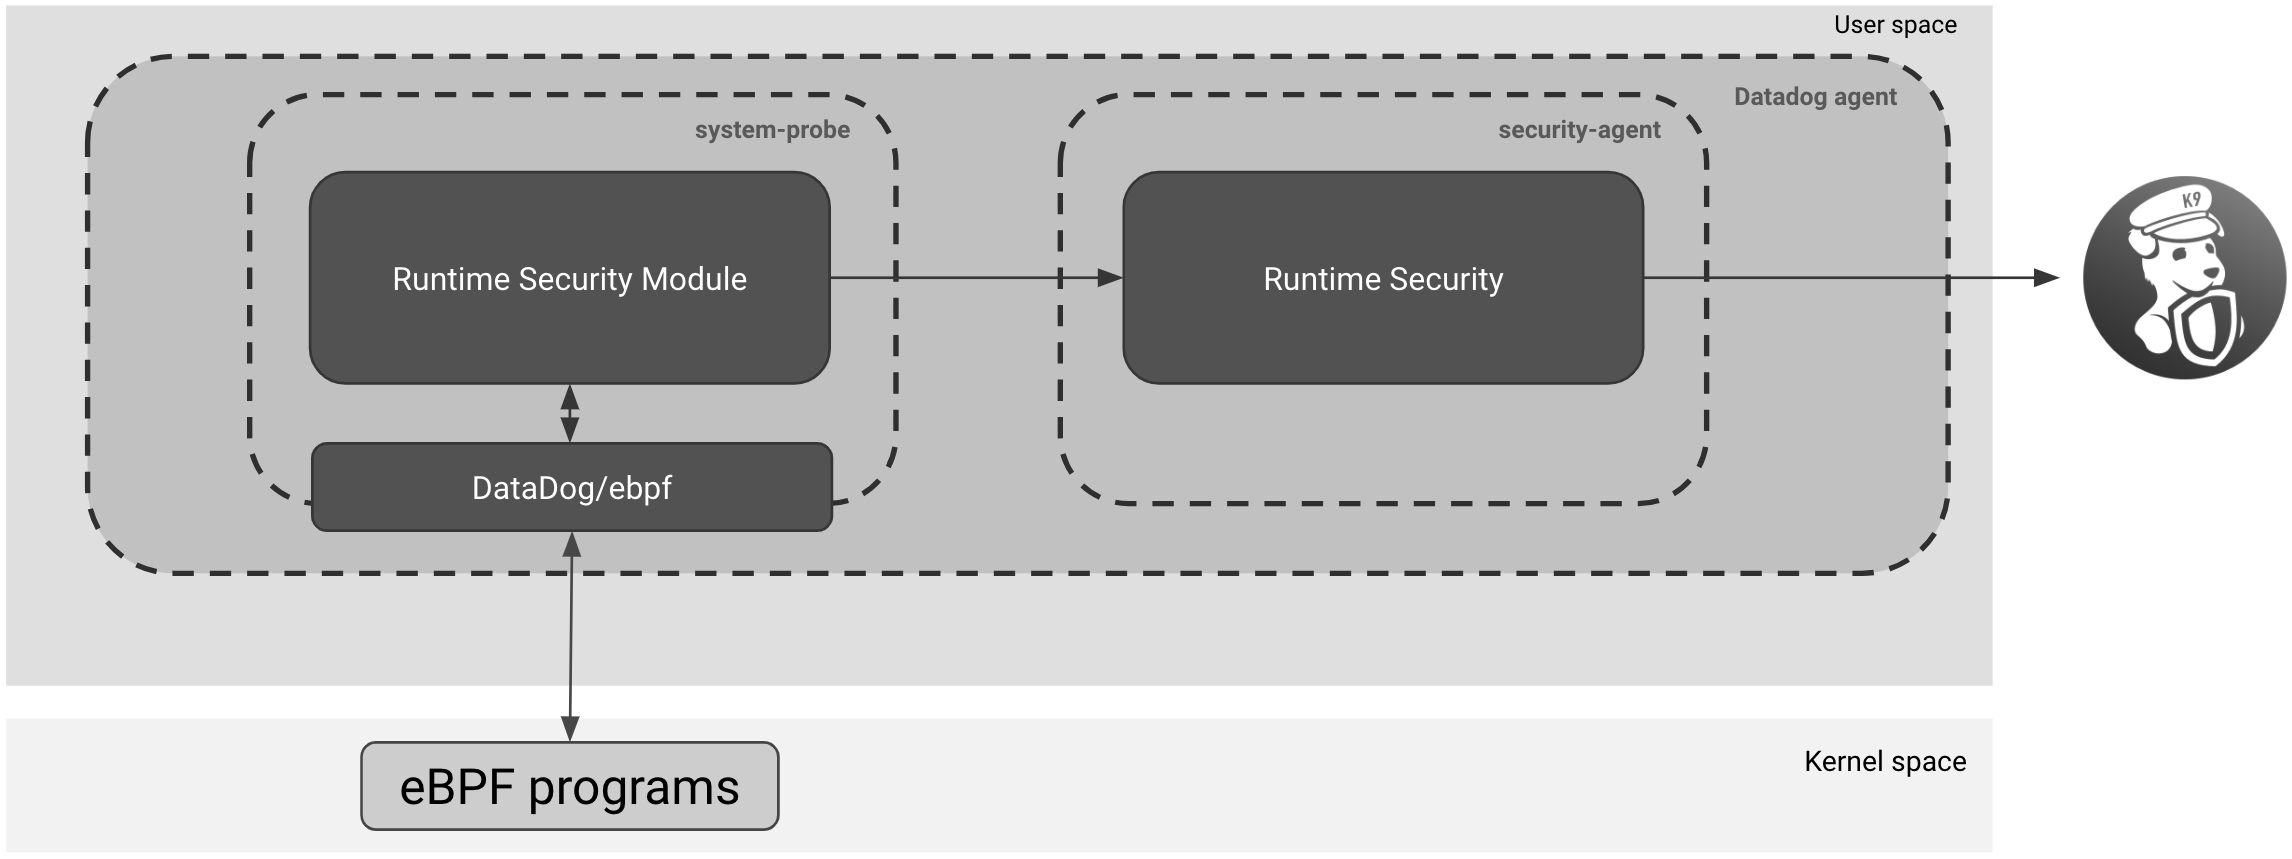
\includegraphics[width=\textwidth]{RuntimeSecurityMonitoringWithEBPF/img/bw-rsa}
  \else
    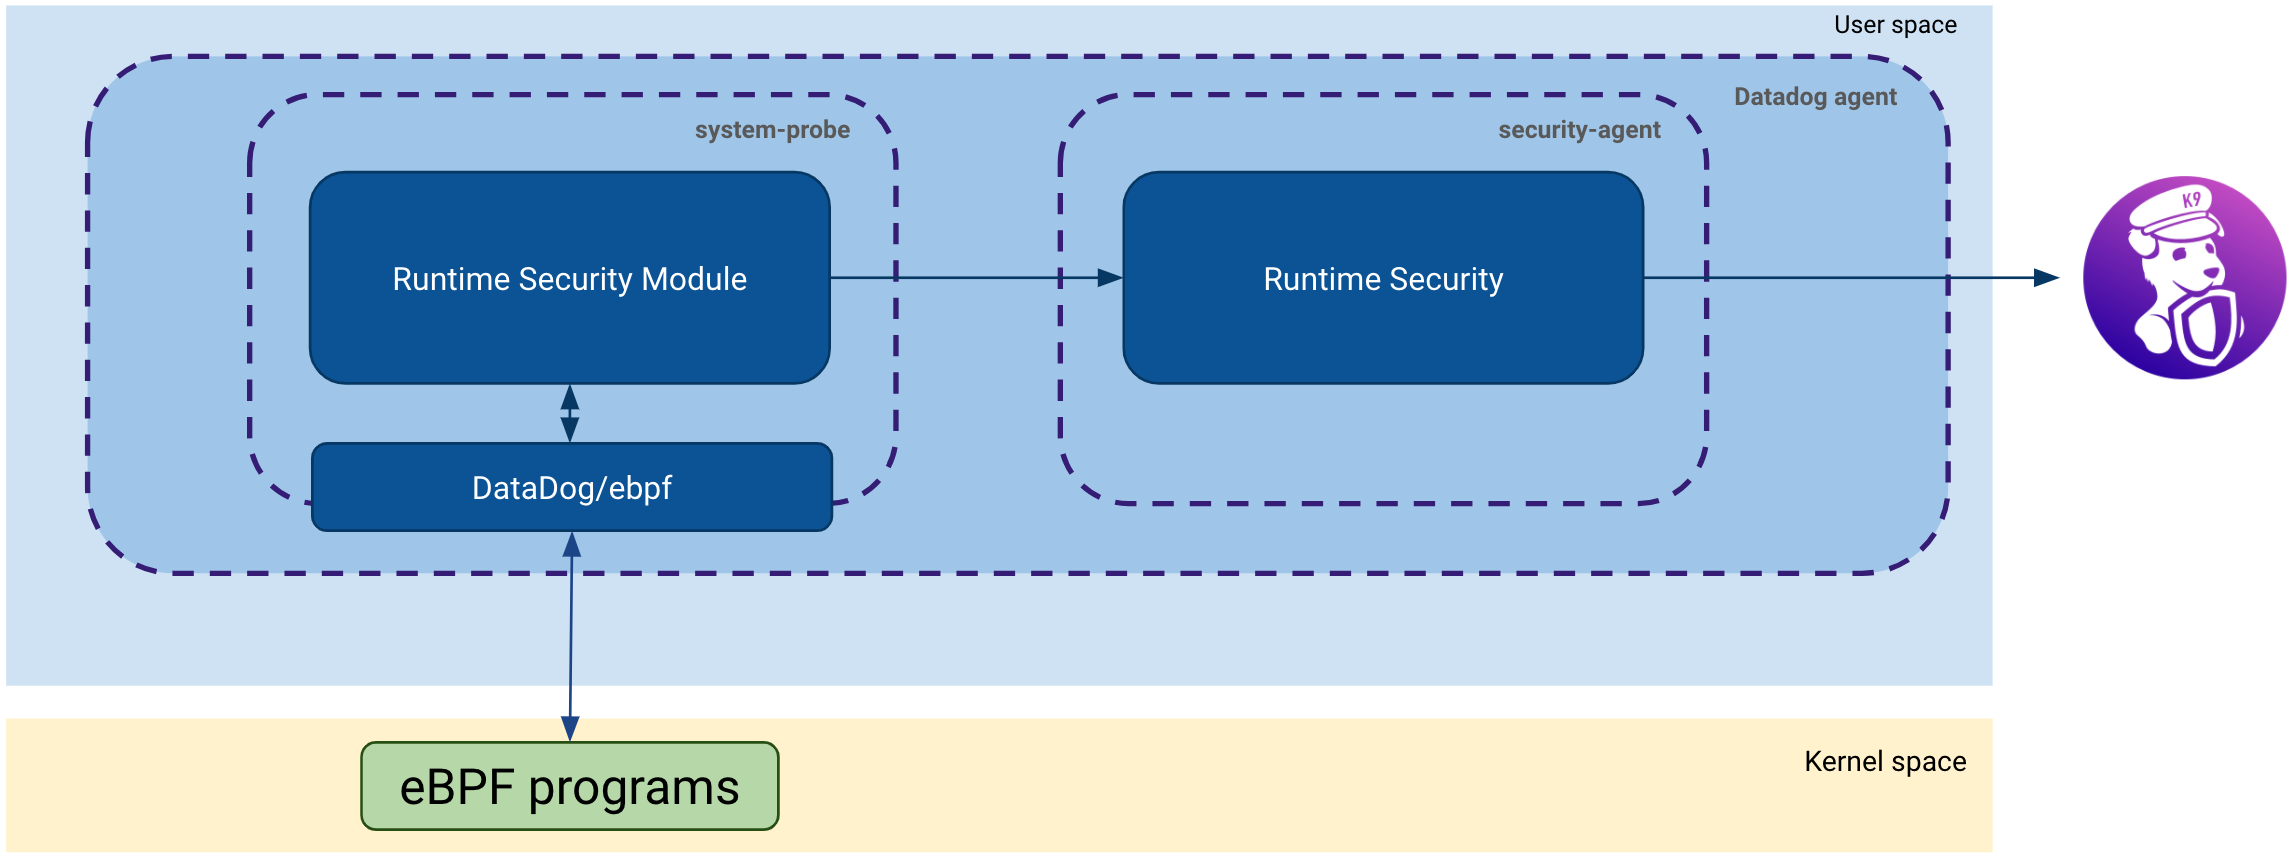
\includegraphics[width=\textwidth]{RuntimeSecurityMonitoringWithEBPF/img/rsa}
  \fi
  \caption{Datadog Runtime Security Agent Architecture}
  \label{fig:RuntimeSecurityMonitoringWithEBPF:RSA}
\end{figure}

The HIDS capabilities of the runtime security agent can be configured through a policy file containing a list of runtime detection rules.
One of the goals of our HIDS was to expose as much context as possible in a way that can easily be used by a security team to detect precise IOCs, and thus write precise detection rules.
This is why we introduced a custom query language called SecL (Security Language) which exposes various kernel events and their context in a simple way.
For example, if you wished to trigger an alert as soon as "/etc/shadow" is opened by a process that isn’t "systemd" or "docker", you could simply write:

\begin{lstlisting}[language={},caption={File integrity monitoring rule example},label={lst:RuntimeSecurityMonitoringWithEBPF:FIMRule}]
open.file.path == "/etc/shadow" && process.file.path not in ["/usr/bin/systemd", "/usr/bin/docker"]
\end{lstlisting}

In other words, SecL lets you write a boolean expression to define your detection rule.
All the process metadata we have access to is available through the \emph{process} keyword.
Similarly, all the container data we collect is available through the \emph{container} keyword.
Overall, the boolean expression can be as complex as you may wish, with file patterns, lists or macros to factorise your rules.
In listing~\ref{lst:RuntimeSecurityMonitoringWithEBPF:FIMRule}, the event that will be assessed by our eBPF programs is the \emph{open} event.
For now, we support 12 event types, that are primarily focussed on the file system (such as \emph{open}, \emph{unlink}, \emph{mkdir}, \emph{link}, \emph{mount} and \emph{umount}, etc), process execution (such as \emph{exec}, \emph{ptrace} etc), or credentials update (\emph{setuid}, \emph{capset}, \emph{chmod}, etc).
However we are actively working on adding new ones in every new release of the Datadog agent.

Performance has also been one of our top priorities, which is why we implemented a dedicated language with a complex mechanism that analyzes the set of rules that you provided in your policy in order to extract two important pieces of information:

\begin{itemize}
  \item The first one is the list of events you care about.
  Your rules might not necessarily require the kernel instrumentation we’ve implemented to support the 12 event types we currently have.
  In other words, in order to minimize our impact on the kernel, we make sure to insert only the probes that we absolutely need.
  \item The second piece of information we extract from your rules is a list of kernel filters that we use to reduce the amount of events sent back to user space.
  In other words, we have implemented an in-kernel pre-filtering feature that is able to understand what you care about and what doesn't even need to be assessed in user space.
  For example, say your set of rules only cares about the "/etc/passwd" file, there is no reason to go back to user space if we detect an event on a file which filename is not "passwd".
  We called this first filtering mechanism an \emph{approver}.
  We also learn at runtime what your workloads are doing, and what can be safely ignored in kernel space based on your set of rules.
  For example, if all the files that you need to watch are in the "/etc/" directory, there is no need to go back to user space with events on files that are in the "/tmp/" directory.
  We called this second filtering mechanism \emph{discarders}.
  To ensure we do not discard events on a file or a process forever, \emph{discarders} can be invalidated at runtime.
  For example, some \emph{discarders} are set with a timeout, so that they will eventually expire.
  We can also decide to remove a \emph{discarder} based on runtime events such as rename or deletion events.
  Similarly, when a mount point is unmounted, we immediately remove the \emph{discarders} that applied to its files.
\end{itemize}

We apply the same filtering logic to the most important attributes exposed in SecL.
This allows us to continuously adapt our in-kernel pre-filtering capabilities to the workload, thus ensuring that our impact on the host remains as low as possible, even if the workloads change over time.

We have also given a particular attention to making sure that the data we collect from kernel space is fully resolved and contextualized.
This means, for example, that file names are not evaluated in kernel space at the syscall level, but much deeper in the file system call path, so that we work with fully resolved and absolute paths.
It also means that we've gone through the long and painful process of checking each kernel version and distribution we support, to make sure that the hook points we chose are stable.

We currently support 2 kinds of rules: file integrity monitoring rules and Process execution monitoring rules.
The Runtime Security Agent is released with a default set of rules~\cite{RuntimeSecurityMonitoringWithEBPF:SecurityAgentPolicies} that you can checkout to better understand its capabilities.

\subsection{File integrity monitoring (FIM)}

File Integrity Monitoring is the ability to detect when a file was created, accessed or modified, thus when its content or attributes changed.
The ability to detect file system changes is a building block of many IOCs.
For example, some dirty cow exploit will try to open the "/etc/passwd" and try to append a line to it.

Apart from IOCs for specific vulnerabilities, File Integrity Monitoring is also very important in general to detect suspicious activity on a host.
For example, an attacker trying to get persistent access to a machine is likely to try to explore a few critical system files to gather information about the host and change its configuration.
"/etc/shadow" and "/etc/passwd" are obvious examples of that, but many other sensitive system files should be monitored.
For example the "authorized\_keys" file of the various users on a host, or the "/etc/resolv.conf" file can both be maliciously accessed to alter the behavior of the host.

As explained in the previous sections, eBPF has multiple limitations which need to be carefully dealt with to avoid bypasses.
Instead of relying on syscall parameters, we actually decided to hook much deeper in the kernel so that we can directly access the \emph{dentry}~\cite{RuntimeSecurityMonitoringWithEBPF:Dentry} tree of the file system.
In a few words, \emph{dentry} structures are used by the kernel to keep track of the tree of files in a file system.
Each "dentry" structure points to an \emph{inode}~\cite{RuntimeSecurityMonitoringWithEBPF:Inode} structure which contains the metadata and all the attributes of a file.
By hooking deep enough in the kernel, we are able to retrieve a pointer to the \emph{dentry} structure of the file that is being modified or accessed for a given event type.
Once we get this \emph{dentry} structure, we know that we have access to the resolved and absolute path of the file, thus preventing any bypass that a syscall based approach would have.

We gave a particular attention to how we chose our kernel hook points.
Given that we target kernels 4.13+ (as well as Centos 7 and 8) we made sure that we do not have any coverage loss because of missing kernel symbols.
We even implemented a safe guard in our eBPF library~\cite{RuntimeSecurityMonitoringWithEBPF:DatadogEBPFLib}: once \emph{system-probe} has started, the eBPF library double checks the list of eBPF programs that were successfully attached to ensure that we are not missing any critical hook points.

All of this hard work eventually paid off, because this ultimately gave us the opportunity to expose an impressive amount of file system context on each alert.
For example, regardless of the event you requested, we are able to expose file metadata like the various modification times, the user, group, access mode of the file and most importantly the mount point of the file system.
Since we also track mount operations at runtime, we are able to fully resolve paths inside containers, and understand the part of the file path that is "inside the container" and the part that was created by your container runtime.
This is a crucial part that is usually missing from legacy runtime security tools, and that allows us to support containers natively.

\subsection{Process execution monitoring}

Process execution monitoring is another building block of runtime security.
In a few words, process execution monitoring can be used to detect processes in your production environment that you didn’t expect to see, or detect execution patterns that should never be seen.
For example, a web server in production should never spawn a shell.
Similarly, you may want to be informed if a package manager is called to install new dependencies on a host.
Looking at the arguments of a call to "curl" can also help you understand what kind of sensitive data an attacker might have stolen.

Another important part of process execution monitoring is the ability to enrich the context we provide with our alerts (regardless of their type).
This is why we’ve spent a lot of time refining a user space process cache that we use to provide the real process tree of each process.
By real process tree, we mean the lineage of all the processes that lead to the one that triggered an alert, regardless if those parent processes are still alive or not.
This is another example of a feature that is missing from most legacy runtime security tools: if you look at the proc file system, you’ll soon realize that when a process dies, its children are immediately attached to the process ID 1.
This means that the kernel loses the lineage context of a process even though it could be a crucial part of context that would tell you which service on a host was exploited.
We’ve introduced the \emph{process.ancestors} selector in our SecL syntax, so that you can write a condition on one of the parents of a process, regardless of the amount of intermediary processes that might have been added to try to fool the detection.
For example, the following rule can be used to detect web shells:

\begin{lstlisting}[language={},caption={Process execution monitoring rule example},label={lst:RuntimeSecurityMonitoringWithEBPF:ProcessRule}]
exec.file.path in ["/bin/bash", "/bin/sh", ...] && process.ancestors.file.path == "/bin/my_web_server"
\end{lstlisting}

Another exciting benefit of hooking deeper in the kernel than the syscall level is the ability to work with pieces of information that are usually not even exposed in user space.
For example, we are able to retrieve the layer of a file in an \emph{overlayfs} filesystem.
This information has powerful security consequences since it can be used to determine if a file, that is about to be executed, was part of the base image of a container, or if it was modified (or simply created) compared to its original version in the base image.
Detecting such a complex use case can be written in one simple rule:

\begin{lstlisting}[language={},caption={In upper layer rule example},label={lst:RuntimeSecurityMonitoringWithEBPF:UppoerLayerRule}]
exec.file.in_upper_layer == true
\end{lstlisting}

Similarly, we are also able to collect process credentials and enrich other events with it.
This means that the full set of user IDs and group IDs, along with kernel capabilities and executable file metadata are collected.
This lets you write interesting rules on processes with dangerously wide access like CAP\_SYS\_ADMIN, or simply detect executions of binary files with the setuid or setgid bit flags set.

\section{Conclusion}

Process monitoring and File integrity monitoring are two important aspects of runtime security, but we are actively working on adding new features to the project in order to extend our detection capabilities.
Thanks to the versatile capabilities of eBPF, the possibilities are almost limitless: from network security monitoring to behavioral analysis, exciting projects are ahead of us !

This paper shows how eBPF can drastically improve the detection capabilities of a runtime security team without having to compromise with performance or coverage.
The ability to surface actionable alerts with comprehensive context about the userspace process and container that triggered the alert, is probably the most important feature that an HIDS can offer in a containerized environment.
During a security incident, quickly identifying the blast radius and the vulnerable parts of the infrastructure will help gain precious minutes and deploy countermeasures in a timely manner.

As shown by the numerous security related initiatives that are making their way into the code base of the eBPF subsystem, we expect to see a growing number of tools use this technology.

\bibliography{RuntimeSecurityMonitoringWithEBPF/biblio}

% Some typography nits
%
% You must not have any space between your text and the \footnote command.
%
% You must add an "espace insécable" ~ before references~\ref{...} and
% citation~\cite{...} commands.
